\documentclass[12pt]{article}
\title{Senior Projects Holography Report}
\date{\today}
\author{Ben Sterling, Dongkyu Kim, Junbum Kim, David Kim}

\usepackage{amsmath}
\usepackage{amssymb}
\usepackage{mathrsfs}
\usepackage{mathtools}
\usepackage{listings}
\usepackage{courier}
\caption
\usepackage[pdftex]{graphicx}
\usepackage{xfrac}
\renewcommand{\baselinestretch}{1.2}


\lstset{basicstyle=\footnotesize\ttfamily,breaklines=true}
\begin{document}
\maketitle
\clearpage

\section{Introduction}
\qquad
Fast prototyping of real-world object has been addressed by many engineers and companies over the past few decades. For instance, 3D printing has especially gained much attention for its practicality. 3D printing has significantly decreased the time required to produce visible and tangible products to a few hours from weeks. On the other end of the spectrum, holography has been attracting attention due to its potentials. This technology, compared to 3D printing, can produce more interactive results at the cost of tangibility. Moreover, holography-based 3D printing is much faster than the traditional 3D printer that builds one microscopic layer at a time, hence reducing the time required to seconds instead of hours,  \cite{Shusteffeaao5496}. These characteristics make holography technology a crucial tool in 3D modeling on its own and also in the context of 3D printing.

However, the application of 3D holography still remains a mystery because of its barriers to the entry. Not only the parts required for the technology are too expensive for easy access, but the theory behind the technology requires a sophisticated understanding of physics for reliable holography projections. These traits make holography very interesting, and successful investigation of the technology will add a great value to the scientific community. In this paper, 3D modeling and holographic projections will be explained to familiarize the audience with the concept to enhance further investigations.

\par
The following sections of the paper are organized as follows. Chapter 2 describes the system pipeline that includes the sampling stage, the digital conversion stage, the transmission stage, and the optical holography projection stage to produce a relatively affordable holographic image of a real-life object. The sampling stage scans a real-world object and stores it digitally on a computer. The digital conversion stage transforms the digitally stored data into a holographic compatible format. The transformed image is then transmitted into the holographic machine called Spatial Light Modulator (SLM). Finally, the optical setup projects the holographic image created by the SLM onto a flat white surface at the projection stage.

\newpage
\section{System Pipeline}

\subsection{Sampling Stage}

\begin{figure}
    \centering
    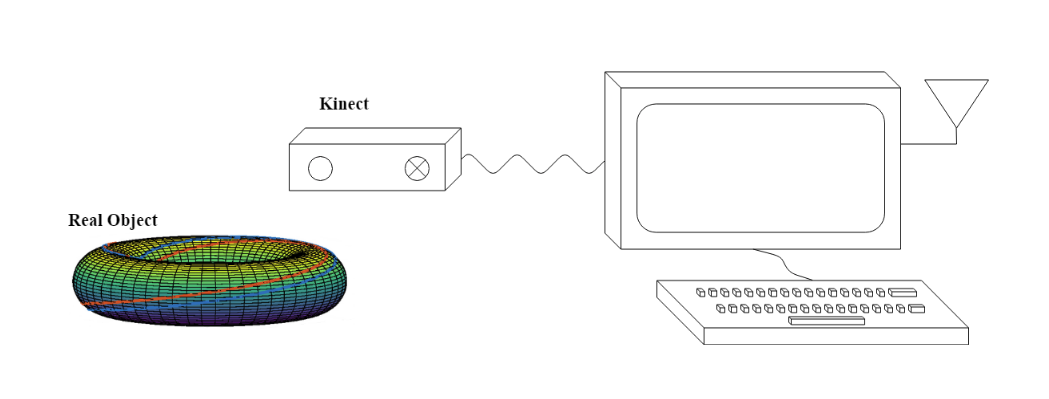
\includegraphics[width=\textwidth]{sampling}
    \caption{Sampling object using Kinect}
    \label{fig:Sampling}
\end{figure}

\qquad
The first stage of the project is sampling a real-world object and storing it into a computer digitally. Since the perception of depth is a crucial part of the 3D holographic projection, it is imperative to sample both the shape and the depth of a real object. In this experiment, Xbox Kinect for Windows Development was used to sample objects. Kinect was originally developed as a module for Xbox to track human motions for entertainment purposes. It can capture an object from a single viewpoint and reconstruct 3D models based on the single viewpoint using a depth sensor and an infrared sensor. In Figure \ref{fig:Sampling}, a hardware connection layout of the sampling stage is shown.

Windows Presentation Foundation (WPF) application was built to communicate the hardware with software. The program was developed using C\# which is the natural platform for the machine. Kinect Studio Version 2.0 and Kinect Software Development Kits were installed to develop the program. Specifically, the KinectFusionExplorer module proved practical for the purpose. The module allows 3D modelling from a single photo shoot from one angle by reconstructing picture from the ordinary camera, the infrared sensor, and the depth sensor. Although the technology cannot provide a 360-degree capture of the sample, this module does reconstruct the sides of the image with only small depth errors. As the Kinect hardware needs information from all three cameras, it requires larger bandwidth compared to other commercial cameras. Hence, USB 3.0 is required to reproduce the program for the extra bandwidth. Features such as shape and depth collected from the Kinect are stored in the computer to later be transformed. More details in what information needs to be encrypted into holographic image will be discussed later. In Figure \ref{fig:kinect}, images created by the camera (left), the depth sensor (top right), and the infrared sensor (bottom right) are shown.

\begin{figure}
    \centering
    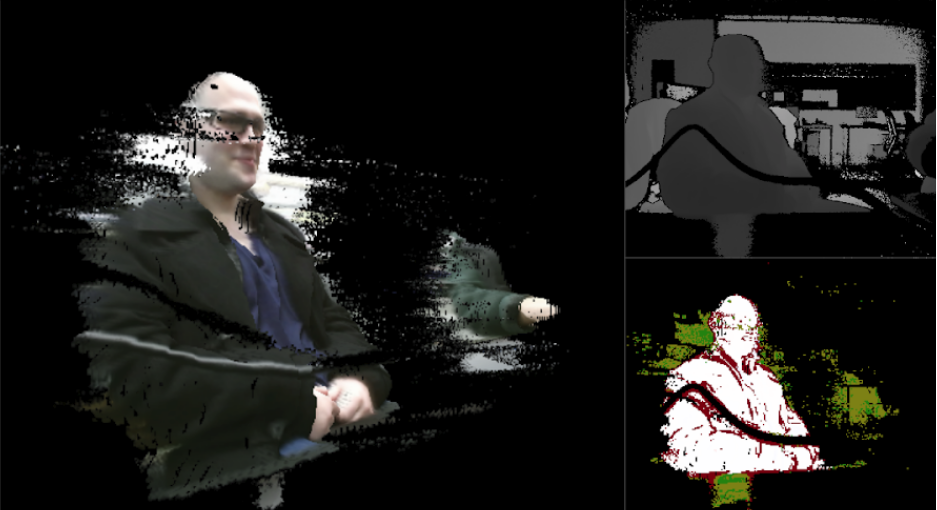
\includegraphics[width=\textwidth]{kinectsample}
    \caption{Sample data obtained from Kinect}
    \label{fig:kinect}
\end{figure}

The WPF application serves two important purposes. Firstly, it provides a user-friendly interface so that the users can use the application without much difficulty. The users can select the thresholds at which they want to set their foreground and background of the sampled data. These would allow users to produce a holographic image without having to know the details of the functionality. Secondly, it allows the integration of different programming modules that is needed for the final product. Specifically, the data extracted from the Kinect need to be converted into a proper usable format, and be sent to the Spatial Light Modulator (SLM). There are existing libraries to transmit data to SLM in python. C\# WPF applications allow users to execute python script on top of the application. To summarize, the application serves as an easy way to integrate software parts while hiding unnecessary details from the end users.

\subsection{Digital Conversion Stage}

The first program that has to run on top of the WPF application transforms the image obtained from the previous sample stage to an SLM compatible format. The SLM that is available for the project is JD9554 spatial light modulator, which is part of Jasper Display's EDKv2 education kit. This modulator is a phase-only modulator, hence the program must convert images into phase masks that contain enough information to reconstruct an image. There are multiple ways of achieving this result, but one of the most efficient and popular approaches for this project is the kinoform method. The kinoform method is based on the observation that when the actual projection occurs, there are random-phase masks applied to the object pattern, making the amplitude of the actual object pattern unimportant. However, according to Poon, the kinoform method without any additional adjustment is very noisy due to its dimension reducing nature \cite{Poon14}. In order to optimize the phase-only holograms, iterative Fourier transform algorithm (IFTA) is used. This algorithm iteratively reduces the error of the reconstructed image by smoothing out the complex amplitude.

In Figure \ref{fig:RMSE}, the root mean square error (RMSE) curve for the reconstruction based on the IFTA algorithm with increasing iteration is shown. The error compares the average of the squared differences between the pixel values of the original image and the image after the reconstruction using the algorithm. There is a big drop in the error from iteration 1 to 4, and a plateau from 4 to 10, and then the error starts to decay again. Each iteration takes about 0.1 seconds, and for the real-time application, doing only 4 loops of IFTA algorithm would be the most beneficial case, as it delivers a reasonable quality in the shortest time. Fig. \ref{fig:images_recon} contains images regarding the experiment with the algorithm. ``peppers.png'' picture was used for the original image which is shown on the top left, and a corresponding phase masks for the SLM was obtained and shown on the top right. Reconstructed images after 2nd and 20th iterations are shown on the bottom left and the bottom right respectively. It is important to note that the phase mask will be the information that will be transferred to the SLM and used to steer the incoming lights to create the hologram.

\begin{figure}
    \centering
    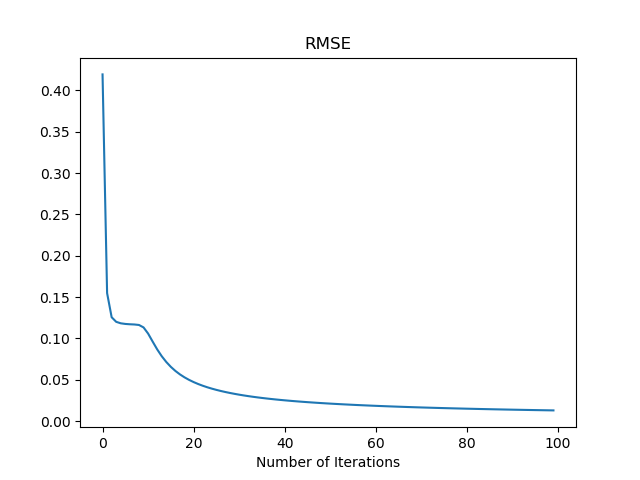
\includegraphics[width=\textwidth]{subroutine2.png}
    \caption{Root Mean Square Error (RMSE) of the Reconstructed Image to the Original Image}
    \label{fig:RMSE}
\end{figure}

\begin{figure}
    \centering
    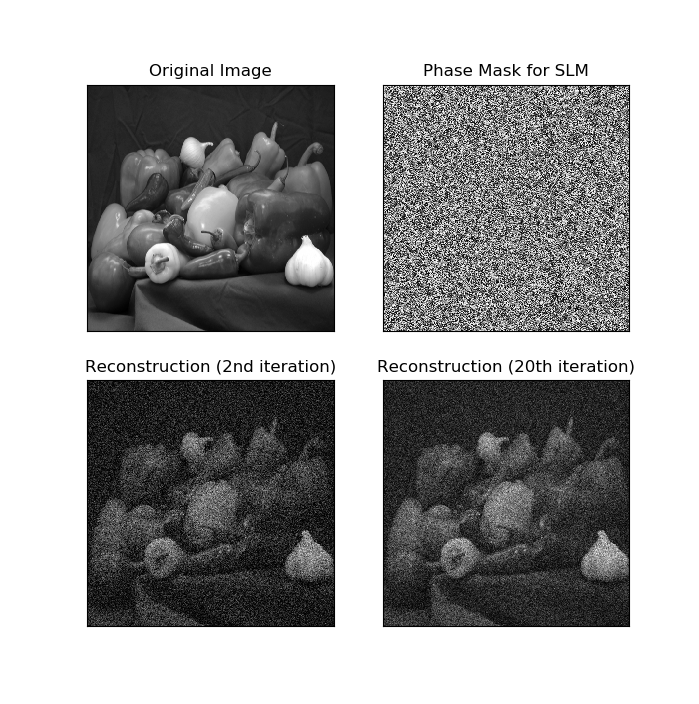
\includegraphics[width=\textwidth]{Result.png}
    \caption{Collection of Images for the Performance Measurement}
    \label{fig:images_recon}
\end{figure}

% Bookmark

\subsection{Digital Projection Stage}

\begin{figure}
    \centering
    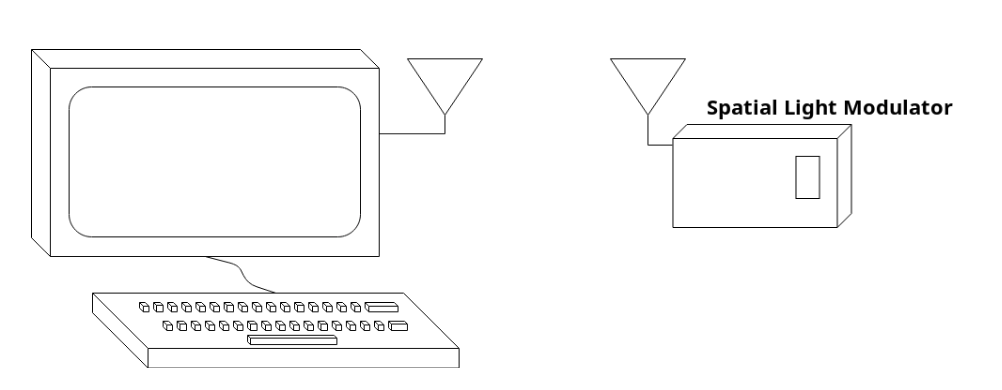
\includegraphics[width=\textwidth]{transmission}
    \caption{Transmitting data from Computer to SLM}
    \label{fig:my_label}
\end{figure}

In the most basic form, SLM can be considered as a monitor that displays image obtained from a computer. The SLM model that we use connects to the computer via an HDMI port. For the manipulation of the image shown on the SLM screen, we use slmPy, a python module created to dynamically control the SLM by Sebastien Popoff \cite{slmPy}. The depth and phase information of the image produced from the digital conversion stage can be sent to the SLM as numpy arrays using the slmPy module. The module has a function that retrieves the resolution of the screen, which may be critical for successful projection of the holography. The depth and phase information is then displayed on the reflective surface of the SLM, which simultaneously is shined by a laser that goes through a beam splitter. The laser that reflects off of the surface will contain the depth and phase information of the image, which subsequently will be projected on a 2D screen as holography.


\section{Holography Background}

\subsection{Wave Fundamentals}

The fundamentals of Holography start from Maxwell's Equations. In the most general case, they are formulated as follows:

\begin{equation}
	\nabla \cdot \vec{D} = \rho\\
\end{equation}

\begin{equation}
	\nabla \cdot \vec{B} = 0
\end{equation}

\begin{equation}
	\nabla \times \vec{H} = \vec{J} + \frac{\partial \vec{D}}{\partial t}
\end{equation}

\begin{equation}
	\nabla \times \vec{E} = -\frac{\partial \vec{B}}{\partial t}
\end{equation}

However, we are interested in utilizing these equations to study optics. Since light waves travel in the air, \(\rho\) = 0 and \(\vec{J}\) = \(\vec{0}\) because there is no source charge or current in the air. Here are the equations we obtain setting sources to zero:

\begin{equation}
	\nabla \cdot \vec{D} = 0
\end{equation}

\begin{equation}
	\nabla \cdot \vec{B} = 0
\end{equation}

\begin{equation}
	\nabla \times \vec{H} = \frac{\partial \vec{D}}{\partial t}
\end{equation}

\begin{equation}
	\nabla \times \vec{E} = -\frac{\partial \vec{B}}{\partial t}
\end{equation}

Lastly, we want to relate D to E, and B to H. The most general relationships that describes these quantities are:

\begin{equation}
	\vec{D} = \epsilon_{0}\vec{E} + \vec{P}
\end{equation}

\begin{equation}
	\vec{B} = \mu_{0}(\vec{H} + \vec{M})
\end{equation}

We assume that all the materials we are working in are Linear, Homogeneous, and Isotropic. The last two equations can be simplified to:

\begin{equation}
	\vec{D} = \epsilon\vec{E}
\end{equation}

\begin{equation}
	\vec{B} = \mu\vec{H}
\end{equation}

where \(\epsilon\) = \(\epsilon_{r}\)\(\epsilon_{0}\) and \(\mu\) = \(\mu_{r}\)\(\mu_{0}\) are constants. If we combine the last two equations along with Maxwell's Equations we get:

\begin{equation}
	\nabla \cdot \vec{E} = 0
\end{equation}

\begin{equation}
	\nabla \cdot \vec{H} = 0
\end{equation}

\begin{equation}
	\nabla \times \vec{H} = \epsilon\frac{\partial E}{\partial t}
\end{equation}

\begin{equation}
	\nabla \times \vec{E} = -\mu\frac{\partial H}{\partial t}
\end{equation}

then we utilize the following identity from vector calculus:

\begin{equation}
	\nabla^2F = \nabla(\nabla \cdot F) - \nabla\times\nabla\times F
\end{equation}

and get:

\begin{equation}
	\nabla^2E - \mu\epsilon\frac{\partial^2 E}{\partial t^2} = 0
\end{equation}

\begin{equation}
	\nabla^2H - \mu\epsilon\frac{\partial^2 H}{\partial t^2} = 0
\end{equation}

The Multi-Dimensional Fourier Transform is defined as follows:

\begin{equation}
	\hat{f} (\vec{k}) = \iint \limits_{R^n}^{} f(\vec{x})e^{-j \vec{k} \cdot \vec{x}} \,d\vec{x}
\end{equation}

and a plane wave is defined as follows:

\begin{equation}
	\vec{E} = \vec{E_{0}}e^{j \omega t - j\vec{k} \cdot \vec{x}}
\end{equation}

Because E and H field are functions of x, y, z, and time, it is possible to span all E and H fields with a superposition of plane waves. This motivates the notation:

\begin{equation}
	\vec{E} = \vec{E_{0}}\psi
\end{equation}

where

\begin{equation}
	\psi = e^{j \omega t - j\vec{k} \cdot \vec{x}}
\end{equation}

Thus, in \(\psi\) notation, the wave equation turns into:

\begin{equation}
	\nabla^2\psi - \mu\epsilon\frac{\partial^2\psi}{\partial t^2} = 0
\end{equation}

\subsection{Plane and Spherical Wave Applications}

For a single frequency, we are interested in the complex amplitude, \(\psi_{p}\) we define as follows:

\begin{equation}
	\psi = \psi_{p}e^{j \omega t}
\end{equation}

We can think of this quantity like the phasor representation of \(\psi\).

The central application of the classical theory is to develop the math behind Fresnel Diffraction. An aperture can be visualized by this diagram:
\begin{center}
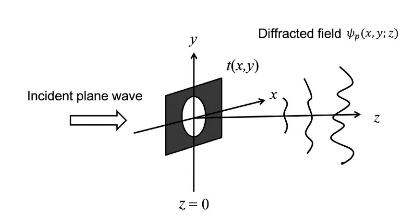
\includegraphics[width=100mm]{tupac5.png}
\end{center}

We also define \(k_{0}\) as the wave number in free space, such that

\begin{equation}
	\nabla^2\psi_{p} + k_{0}^2\psi_{p} = 0
\end{equation}

since

\begin{equation}
	\lambda f = c \rightarrow k_{0} = \omega/c
\end{equation}

By considering the incoming plane wave as a superposition of plane waves (like we did with the Multi-Dimensional Fourier Transform), we obtain the result:

\begin{equation}
	\mathscr{F} \Big\{ \frac{\partial^2 \psi_{p}}{\partial x^2} \Big\} = (-jk_{x})^2\Psi_{p} = -k_{x}^2\Psi_{p}
\end{equation}

and

\begin{equation}
	\mathscr{F} \Big\{ \frac{\partial^2 \psi_{p}}{\partial y^2} \Big\} = (-jk_{y})^2\Psi_{p} = -k_{y}^2\Psi_{p}
\end{equation}

where

\begin{equation}
	\Psi_{p} = \mathscr{F} \{\psi_{p}\}
\end{equation}

Finally, if we take the Fourier Transform of both sides of (26) we obtain:

\begin{equation}
	\frac{\partial^2\Psi_{p}}{\partial z^2} + k_{0}^{2} \bigg ( 1 - \frac{k_{x}^2}{k_{0}^2} - \frac{k_{y}^2}{k_{0}^2} \bigg ) \Psi_{p} = 0
\end{equation}

While this looks complicated, it is really only an Ordinary Differential Equation of \(\Psi_{p}\) with respect to z. It's solution is:

\begin{equation}
	\Psi_{p} = \big(\Psi_{p}\vert_{z = 0}\big) exp\Bigg(-jk_{0}z\sqrt{1 - \frac{k_{x}^2}{k_{0}^2} - \frac{k_{y}^2}{k_{0}^2}}\Bigg)
\end{equation}

If we let

\begin{equation}
	\Psi_{p0} = \big(\Psi_{p}\vert_{z = 0}\big)
\end{equation}

Then we can recognize the solution in (32) as a transfer function. We define:

\begin{equation}
	\mathscr{H} = \frac{\Psi_{p}}{\Psi_{p0}} = exp\Bigg(-jk_{0}z\sqrt{1 - \frac{k_{x}^2}{k_{0}^2} - \frac{k_{y}^2}{k_{0}^2}}\Bigg)
\end{equation}

\(\mathscr{H}\) is called the Spatial Frequency Transfer Function of Propagation. It applies to our specific apparatus under consideration and describes Fresnel Diffraction of the output of a plane wave hitting an aperture. \(\psi_{p0}\) is the function controlled by the shape of the aperture; if this equals \(\delta(x,y)\), for example, then the output of the aperture is purely the Spatial Frequency Transfer Function response, because this is equivalent to convolving with a delta in 2-Dimensions, returning \(\mathscr{F}^{-1} \{\mathscr{H}\} \) in the time domain.

\subsubsection{Fresnel Diffraction}

We have \(\mathscr{H}\), but more often than not, the traveling waves make very small angles from the normal direction of the aperture. This allows us to utilize the Paraxial Approximation:

\begin{equation}
	\sqrt{1 - \frac{k_{x}^2}{k_{0}^2} - \frac{k_{y}^2}{k_0^2}} \approx 1 - \frac{k_{x}^2}{2k_{0}^2} - \frac{k_{y}^2}{2k_{0}^2}
\end{equation}

Once we apply this approximation, the Spatial Frequency Transfer Function of Propagation simplifies:

\begin{equation}
	\mathscr{H} = exp(-jk_{0}z)exp\bigg[\frac{j(k_{x}^2 + k_{y}^2)z}{2k_{0}}\bigg]
\end{equation}

In this specific example, we are using the Two Dimensional Fourier Transform (z remains constant):

\begin{equation}
	\Psi_{p}(k_{x},k_{y},z) = \iint \limits_{R^2}^{} \psi_{p}(x,y,z)e^{-jk_{x}x - jk_{y}} \,dx\,dy
\end{equation}

Thus we get the Spatial Impulse Response, h:

\begin{equation}
	h(x,y,z) = \mathscr{F}^{-1}\{\mathscr{H}\} = \frac{jk_{0}}{2\pi z} exp(-jk_{0}z)exp\bigg[\frac{-jk_{0}(x^2 + y^2)}{2z}\bigg]
\end{equation}

\subsection{Holography Fundamentals}

The simplest holography setup, and a good starting point to understanding the subject, is this collection of Fresnel Plates:

\begin{center}
	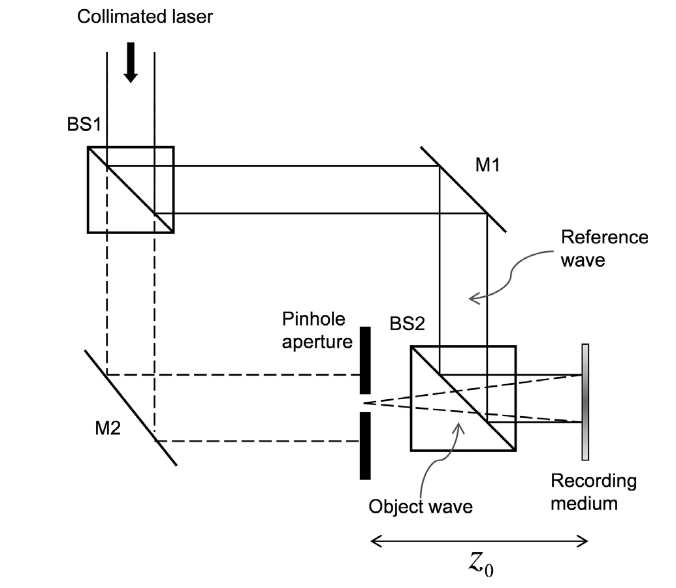
\includegraphics[width=100mm]{tupac7.png}
\end{center}

First, we use a collimated laser so that the direction of propagation of each wave is parallel.
The first beam splitter (BS1) divides the laser in two paths of equal power, one will be used as a reference and the other contains the object information.
We recombine the waves at the second beam splitter (BS2). If the object wave is denoted as \(\psi_{0}\) and the reference wave is \(\psi_{r}\).
Since our aperture is a pinhole, our input function (referencing the Spatial Frequency Transfer Function) is \(\delta(x,y)\), thus:

\begin{equation}
	\begin{multlined}
		\psi_{0}(x,y,z_{0}) = \delta(x,y) * h(x,y,z_{0}) = h(x,y,z_{0})
		\\= exp(-jk_{0}z_{0})\frac{jk_{0}}{2\pi z_{0}}exp\bigg[\frac{-jk_{0}(x^2 + y^2)^2}{2z_{0}}\bigg]
	\end{multlined}
\end{equation}

and \(\psi_{r}\) is just a plane wave propagating in the \(z_{0}\) direction:

\begin{equation}
	\psi_{r} = a\,exp(-jk_{0}z_{0})
\end{equation}

It is important to note that the light intensity is proportional to square of the complex amplitude, I(x,y) \(\propto\) \(|\psi_{p}(x,y)|^2\).
Thus we define transmittance, t(x,y) as:

\begin{equation}
	t(x,y) = |\psi_{p}(x,y)|^2
\end{equation}

For our specific case:

\begin{equation}
	\begin{multlined}
	t(x,y) = |\psi_{o}(x,y) + \psi_{r}(x,y)|^2
	=(\psi_{o} + \psi_{r})(\psi_{o} + \psi_{r})^*
	\\= a^2 + (\frac{k_{0}^2}{2\pi z_{0}})^2 - \frac{-jk_{0}a}{2\pi z_{0}}
	exp\bigg[ \frac{jk_{0}}{2z_{0}}(x^2 + y^2) \bigg] +
	\\\frac{-jk_{0}a}{2\pi z_{0}}
	\exp\bigg[\frac{-jk_{0}}{2z_{0}}(x^2 + y^2) \bigg]
	\end{multlined}
\end{equation}

We can recognize the sine function inside the last line:

\begin{equation}
	t(x,y) = a^2 + \big(\frac{k_{0}}{2\pi z_{0}}\big)^2 +
	\frac{ak_{0}}{\pi z_{0}}sin\bigg[\frac{k_{0}}{2z_{0}}(x^2 + y^2)\bigg]
\end{equation}

And thus, we can observe the diffraction pattern of this aperture as follows:

\begin{center}
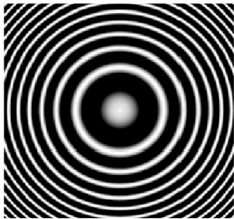
\includegraphics[width=50mm]{tupac8.png}
\end{center}

By inspection, the output of the machine obeys a sinusoidal pattern, with some DC value in towards the center (x = 0 and y = 0), and the frequency
of the sinusoid increases parabolically moving radially outward.
Also, for any tangent vector \(v_{p}\), the spatial frequency is defined as the directional derivative of the angle:

\begin{equation}
	v_{p}\bigg[ \frac{k_{0}(x^2 + y^2)}{2z_{0}} \bigg] = \frac{k_{0}}{z_{0}}(v_{1}p_{1} + v_{2}p_{2}), \forall v_{p} \in T_{p} \mathbb{R}^2
\end{equation}

This result is more significant in differential form:

\begin{equation}
	d \bigg( \frac{k_{0}(x^2 + y^2)}{2z_{0}} \bigg) = \frac{k_{0}}{z_{0}}(xdx + ydy)
\end{equation}

The frequency increases linearly in any direction of our choosing.
It is important to note that an observer at a distance will see the following
\(\psi_{rec}\) instead because they are at a distance, z, away from the
recording medium.

\begin{equation}
	\psi_{p} = \psi_{rec}t(x,y)*h(x,y,z)
\end{equation}

Where \(\psi_{rec}\) is the field on the projecting surface.

\subsubsection{3D Holographic Imaging}

In this next section, we wish to identify the effects of different co-planar displacements
(x and y) and different distances from the medium (z). We can visualize this problem with the following diagrams:

\begin{center}
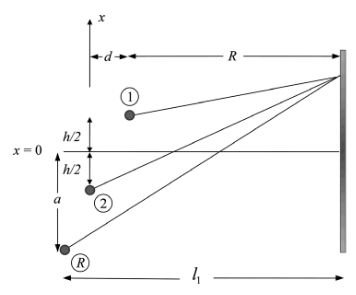
\includegraphics[width=100mm]{tupac11.png}
\end{center}

\begin{center}
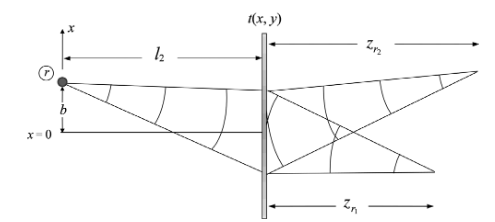
\includegraphics[width=100mm]{tupac12.png}
\end{center}

The first graph displays two source points with a reference wave R, and the second displays the reconstructed point r (the location a viewer SEE'S the object).

The following identity under convolution helps to simplify the upcoming calculations.

\begin{equation}
	\delta(x - \alpha,y - \beta)*h(x,y,z) = \delta(x,y)*h(x - \alpha,y - \beta,z)
\end{equation}

The physical significance of this identity is that being off-center from the pinhole
aperture is equivalent to translating the center Spatial Impulse Response: a very important property.

Thus, we can find the three relevant complex fields as follows:

\begin{equation}
	\psi_{p1} = \delta(x - \frac{h}{2},y)*h(x,y,R) = h(x - \frac{h}{2},y,R)
\end{equation}

\begin{equation}
	\psi_{p2} = \delta(x + \frac{h}{2},y)*h(x,y,R + d) =
	h(x - \frac{h}{2},y,R + d)
\end{equation}

\begin{equation}
	\psi_{pR} = \delta(x + a,y)*h(x,y,l_{1}) = h(x + a,y,l_{1})
\end{equation}

Now, the intensity can be found as follows (by definition)

\begin{equation}
	\begin{multlined}
	t(x,y) = |\psi_{p1} + \psi_{p2} + \psi_{pR}|^2
	\\ (\psi_{p1} + \psi_{p2} + \psi_{pR})(\psi_{p1} + \psi_{p2} + \psi_{pR})^*
	\end{multlined}
\end{equation}

Each \(\psi_{pi}\psi_{pi}^*\) for \(i \in \mathbb{Z}^+\) is not very interesting, because the wave parts cancel and they are just zeroth order waves.
Also, note \(\psi_{pi}\psi_{pj}^* = (\psi_{pj}\psi_{pi}^*)^* \), so we only need three transmittances to determine the intensity

If we take one transmittance:

\begin{equation}
	t_{rel1}(x,y) = \psi_{p1}^*\psi_{pR}(x,y) = exp(\frac{jk_{0}}{2R}[(x - \frac{h}{2})^2 + y^2])exp(\frac{-jk_{0}}{2R}[(x + a)^2 + y^2])
\end{equation}

and then solve for the reflected \(\psi\), we get:

\begin{equation}
	\psi_{pr}(x,y)t_{rel1}(x,y)*h(x,y,z)
\end{equation}

Where:
\begin{equation}
	\psi_{pr} = \delta(x - b,y)*h(x,y,l_{2}) = h(x - b,y,l_{2})
\end{equation}

This must be true because INDEPENDENT of the points 1 and 2, the field is being
affected by a plane wave coming from the reconstruction point. Thus, if we want to
approximate the reflected wave, it is given by:

\begin{equation}
	\begin{multlined}
	\psi_{ref} \propto exp\bigg(\frac{-jk_{0}}{2l_{2}}[(x - b)^2 + y^2]\bigg)
	exp\bigg(\frac{-jk_{0}}{2R}[(x - \frac{h}{2})^2 + y^2]\bigg)
	\\exp\bigg(\frac{-jk_{0}}{2l_{1}}[(x + a)^2 + y^2]\bigg)
	*\frac{jk_{0}}{2\pi z}exp\bigg(\frac{-jk_{0}}{2z}[x^2 + y^2]\bigg)
	\end{multlined}
\end{equation}

At this point in the derivation, we must remember the definition of 2D convolution we are working with:

\begin{equation}
	\big(f_{1}*f_{2}\big)(x,y) = \iint \limits_{R^2}^{} f_{1}(x',y')f_{2}(x - x',y - y') \,dx'\,dy'
\end{equation}

By far the most confusing part of this derivation: the coefficients in front of \(x'^2\) and \(y'^2\) must equal zero because the convolution in (55) must evaluate to a \(\delta\) function.
Think of it this way: If it did not evaluate to a \(\delta\), this would imply the field has multiple non-zero space values for a single image point; we do not allow a single point
to spread into a cloud, this would violate our empirical observations.

Thus by inspection, we derive the equation:

\begin{equation}
	\frac{1}{R} - \frac{1}{l_{1}} - \frac{1}{l_{2}} - \frac{1}{z_{r1}} = 0
\end{equation}

Through very tedious math, we get that:

\begin{equation}
	\psi_{ref} \propto \delta \bigg[ x + z_{r1}\bigg(
	\frac{b}{l_{2}} - \frac{h}{2R} - \frac{a}{l_{1}}\bigg),y\bigg]
\end{equation}

Similarly for the second point:

\begin{equation}
	\frac{1}{R + d} - \frac{1}{l_{1}} - \frac{1}{l_{2}} - \frac{1}{z_{r2}} = 0
\end{equation}

\begin{equation}
        \psi_{ref} \propto \delta \bigg[ x + z_{r2}\bigg(
        \frac{b}{l_{2}} - \frac{h}{2(R + d)} - \frac{a}{l_{1}}\bigg),y\bigg]
\end{equation}

These equations are the starting point to understanding magnification and translation distortion of images.
For the most part, we are simplifying the problem of displaying an image to
effects between two points.

\subsubsection{Holographic Magnification}

In this context, magnification is defined as:

\begin{equation}
	M_{Long}^r = \frac{z_{r2} - z_{r1}}{d}
\end{equation}

This is literally a ratio of the hologram depth over the real depth between these two points.

We substitute from equation (57) and (59) (Assuming: R \(\gg\) d)

\begin{equation}
	M_{Long}^r = \bigg(\frac{l_{1}l_{2}}{l_{1}l_{2} - Rl_{1} - Rl_{2}}\bigg)^2
\end{equation}

We define lateral magnification as the difference in x virtual positions over the real x distance (h). We use equations (58) and (60):

\begin{equation}
	\begin{multlined}
		M_{Lat}^r = \frac{z_{r2}\bigg( \frac{b}{l_{2}} + \frac{h}{2(R + d)} - \frac{a}{l_{1}}\bigg) - z_{r1}\bigg(\frac{b}{l_{2}} - \frac{h}{2R} - \frac{a}{l_{1}} \bigg)}{h}
		\\\approx \frac{(z_{r2} - z_{r1})\bigg(\frac{b}{l_{2}} -\frac{a}{l_{1}} \bigg) + (z_{r2} + z_{r1})\frac{h}{2R}}{h}
	\end{multlined}
\end{equation}

assuming \(R \gg d\)

If we align the points in a special way such that:

\begin{equation}
	\frac{b}{l_{2}} - \frac{a}{l_{1}} = 0
\end{equation}

We get the fascinating result that

\begin{equation}
	M_{Long}^r = (M_{Lat}^r)^2
\end{equation}

\subsubsection{Holographic Translation}

The equation for Lateral Magnification gives us the distortion between two holographic points if (64) is not met:

\begin{equation}
	\Delta x = x_{1} - x_{2} = (z_{r2} - z_{r1})\bigg(\frac{b}{l_{2}} - \frac{a}{l_{1}}\bigg)
\end{equation}

This figure shows how an artificial \(\Delta x\) comes about from erroneous orientation

\begin{center}
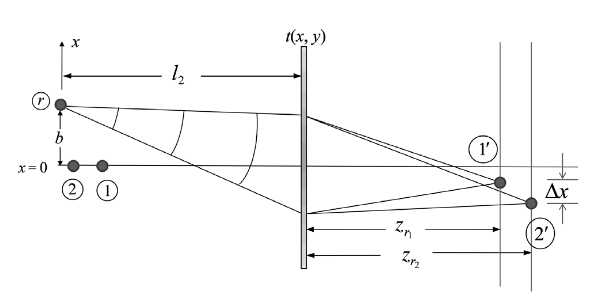
\includegraphics[width=100mm]{tupac13.png}
\end{center}

\subsubsection{Off-Axis Holography}

The standard holography setup we have studied is called on-axis holography.
The only problem with this approach is that we get twin images when we expand
the full equation for transmittance: (the conjugation terms make the twin images)

\begin{equation}
	t(x,y) = |\psi_{r} + \psi_{o}|^2 = |\psi_{r}|^2 + |\psi_{o}|^2
	 + \psi_{r}^*\psi_{o} + \psi_{r}\psi_{o}^*
\end{equation}

Off-Axis holography takes care of this problem by introducing the reference
light at an angle \(\theta\)

\begin{center}
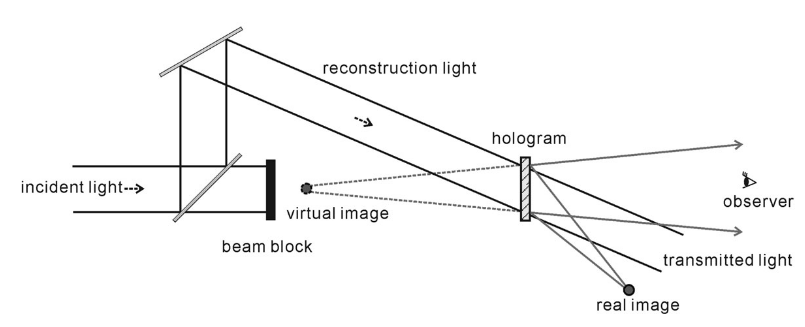
\includegraphics[width=100mm]{tupac9.png}
\end{center}

We can redo the logic of equation (67) as follows (the extra phase factor comes
out from the extra distance the reference wave needs to travel)

\begin{equation}
	\begin{multlined}
	t(x,y) = |\psi_{r}e^{jk_{0}sin\theta x} + \psi_{o}|^2 = |\psi_{r}|^2 + |\psi_{o}|^2
         + \psi_{r}^*\psi_{o}e^{-jk_{0}sin(\theta) x} + \psi_{r}\psi_{o}^*e^{jk_{0}sin(\theta)x}
	\\=|\psi_{r}|^2 + |\psi_{o}|^2 + 2|\psi_{0}^*\psi_{r}|cos(2\pi f_{x}x + \phi (x,y))
	\end{multlined}
\end{equation}

The phase getting scaled by \(xsin(\theta)\) makes sense because at \(\theta = \pi/2\), the extra distance turns into just x, and at \(\theta = 0\)
the reference wave is already in phase with the object wave, so no adjustment would be necessary. Just like the earlier section,
we recognize the cosine identity in the top of the last equation (the \(\phi\) is any extra phase that came from the \(\psi_{o}\) \(\psi_{r}\) pair not counting
the angle \(\theta\)). Specifically, \(f_{x} = \frac{sin(\theta)}{\lambda}\).

Finally, we need to factor in the reconstruction light. If it has the same magnitude and direction
as the reference light, we can represent it with the following wave function (which
later gets convolved with h(x,y,z) to render the real image):

\begin{equation}
	\begin{multlined}
	\psi = \psi_{r}e^{jk_{0}sin(\theta)x}t(x,y)
	\\=|\psi_{r}|^2\psi_{r}e^{jk_{0}sin(\theta)x} + |\psi_{0}|^2\psi_{r}e^{jk_{0}sin(\theta)x}
	\\+ \psi_{o}|\psi_{r}|^2 + \psi_{o}^*\psi_{r}^2e^{2jk_{0}sin(\theta)x}
	\end{multlined}
\end{equation}

\begin{center}
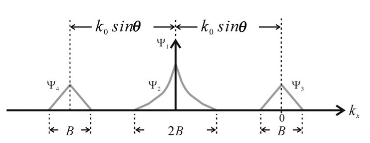
\includegraphics[width=100mm]{tupac14.png}
\end{center}

Upon closer examination, we can regard \(k_{0}sin(\theta)\) our carrier frequency (in radians). Since \(\psi_{r}\) is a reference light, it is entirely DC, so the first term
in (69) is \(\Psi_{1}\), the carrier.
The second term in (69) is \(\Psi_{2}\) because the phasor convolves the magnitude-squared of the object wave out to the carrier frequency.
The third (and most important) term, \(\Psi_{3}\) is the only one that is not modulated by the carrier (it gets cancels out by the algebra).
This is the only term that is visible to the human eye!

By inspection, the minimal angle \(\theta\) we need to prevent aliasing can be given by:

\begin{equation}
	k_{0}sin(\theta) \geq \frac{3B}{2}
\end{equation}

\section{Project Setup}

\begin{center}
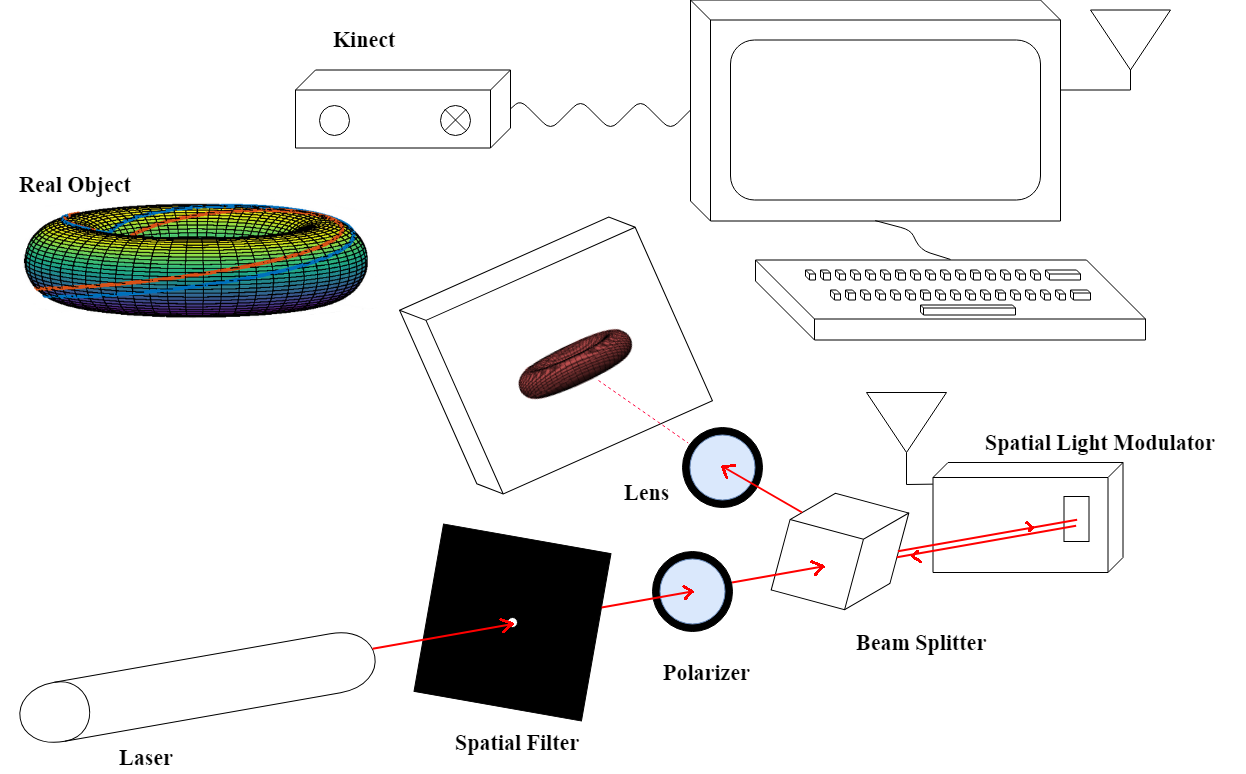
\includegraphics[width=100mm]{tupac10.png}
\end{center}

This is a picture of our Hollistic project. the software component is on top as described before. We start on the bottom left corner with a coherent laser source; it is important that the laser is coherent otherwise random phase artifacts would be introduced from the start further degrading the quality of the final hologram. We next use a pinhole apparatus to filter out the higher order noise artifacts that might have been introduced by the laser and surrounding distance; this also centers the laser by converting the incoming plane wave of the laser into a spherical wave (which turns into a plane wave again after applying the Paraxial Approximation). We also put a polarizer in front of the pinhole so that the light incoming into the SLM has the anticipated linear polarization that it expects (the wrong polarization may not reflect off the SLM as expected).

We put a beam splitter in front of the polarizer to send half of the incoming beam onto the screen and half to the SLM. The SLM is electronically steered by the incoming video signal, and has 8 bit precision in the phase of the wave that it reflects. An important note is that the wave reflected off the SLM occupies the same physical space as the incoming wave: this works due to Transmission Line Theory (the two waves do not interfere with one another; they are governed only by Maxwell's Equations). Finally, the reflected wave goes into the beam splitter and sums with the incident light as both waves travel to the recording medium. This is how our hologram appears on the screen.

\section{List of Materials}

We are using a JD9554 Spatial Light Modulator, a P20S 20 micro-meter pinhole from Thorlabs, a BS013 Cube Beam Splitter, AL2520-A collimated lenses, C560TME-B Aspheric Lens, an LPVISE200-A Polarizer, and a high powered laser

\section{Physical Setup}
At the very end of the first semester, we recieved all the parts needed to finish the SLM setup. The problem was that we knew the order in which to place the parts, but we didn't know what precision we needed to get the hologram working. In addition, the parts we had ordered did not fit very well into the holders that came with the optical board, we did not know if our laser was powerful enough to generate the hologram, and we could barely get any light to come out of our pinhole (it is a very delicate component).

In the meantime, we decided to ask Professor Wolf for advice (he has the most Holography experience). [TODO: David]. The most important take-away we learned was that our 10mW laser was powerful enough to produce the hologram we wanted.

Even though it was not ideal, we designed parts to be 3D printed to raise our components off the board by a precise height. To make them general purpose, we designed a three piece system consisting of a base, hexoganol shaft, and insert piece that could be hand-tightened by a screw:

\begin{center}
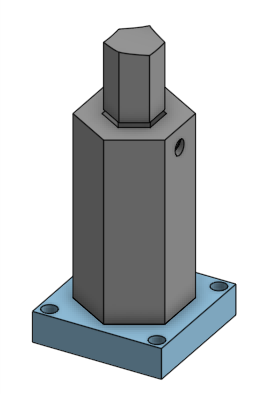
\includegraphics[width=100mm]{holder.png}
\end{center}

We were planning to make about 6 of these to precisely place the laser, collimating lense, pinhole, and polarizers, but got very lucky when we tried to investigate which piece was "most important". Once we removed the pinhole and tried the collimating lense on a stand by itself, a much wider beam of light was produced. We tried to see if would produce any noticeable pattern, but figured out the reflected light was not combining with the reference light correctly because the beam splitter's angle was slightly off. We used the precision handles to fix it and noticed the SLM produced an interesting pattern:

\begin{center}
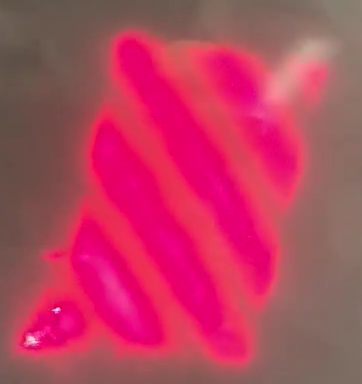
\includegraphics[width=100mm]{initHologram.png}
\end{center}

We saw this switching pattern from diagonal lines to vertical lines when the SLM was on without video input. As soon as we connected the HDMI port to Jun's computer, we were able to see very noisy images he sent to the display. Here is an example of Ben's face:

\begin{center}
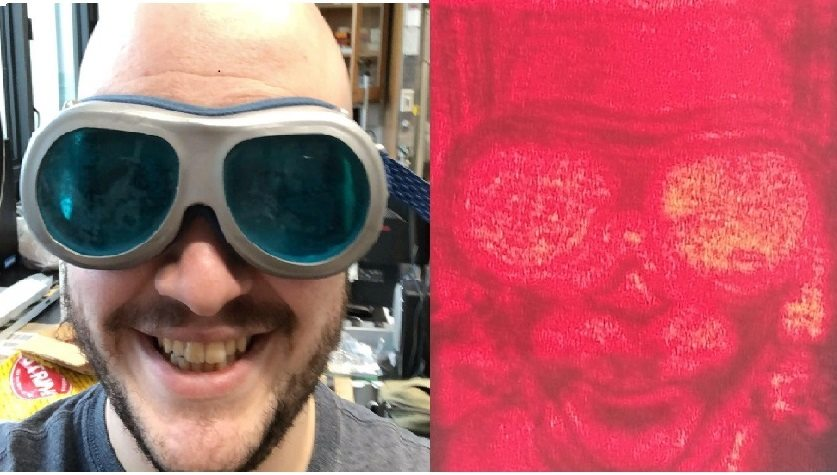
\includegraphics[width=100mm]{noisy_hologram.jpg}
\end{center}

Finally, we noticed that the polarizer made a reduction in noise, but it was not an essential piece we needed to produce an image. We also figured out that our laser is horizontally polarized because rotating our polarizer by 90 degrees completely blocked the laser's light.

\section{Why we couldn't achieve "real" 3D}

[TODO: Dongkyu]

Instead of using a crystal, we decided to utilize a cross-eyed hologram; this works by displaying the right and left eyed images in front of the opposite eye so that the viewer crosses their eyes and sees a 3D image (by illusion).

\section{Stereoscopic Pair Generation}

At this stage, we had developed the WPF application to obtain a color/depth map and immidiately send it to the SLM, but needed to figure out how to convert color/depth information to right and left eyed views (the stereoscopic pair). We tried to find a library to do this conversion, but most (in particular OpenCV) provided libraries to solve the opposite problem (converting a stereoscopic pair to a color/depth map). Upon further examination, we determined our problem could be solved with simple geometry, so we came up with the following solution:

\begin{center}
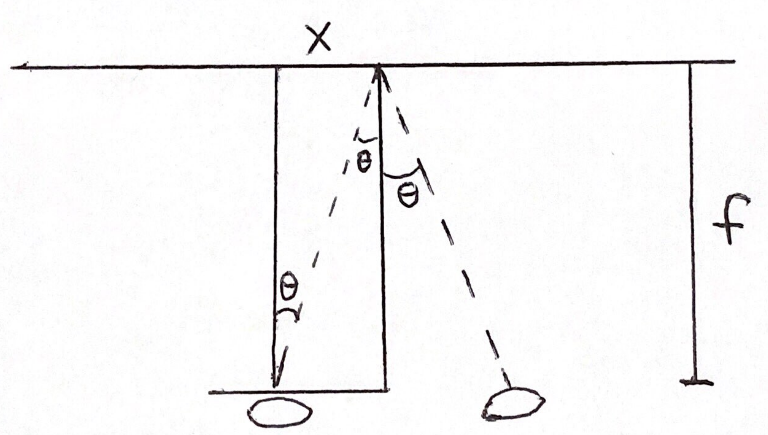
\includegraphics[width=100mm]{eye_disp_pic.png}
\end{center}

To create the image pair, we need to find how far each eye is from the center, then dilate pixels accordingly. To get eye distance, we assume a certain focal distance (f), eye-angle (\(\theta\)), and pixel density (D); the pairs are not highly sensitive to these parameters because the viewer can adjust depth as needed (with the use of their finger) but we needed reasonable values, so we chose f = 2, \(\theta\) = \sfrac{\(\pi\)}{6}, and D = 75. We need to solve for x in the picture. Using basic trig and scaling by our pixel density, we get: \[x = Df\tan(\theta)\]

Next, we need to dilate each pixel depending on its depth (given by the depth map) and distance from the eye:

\begin{center}
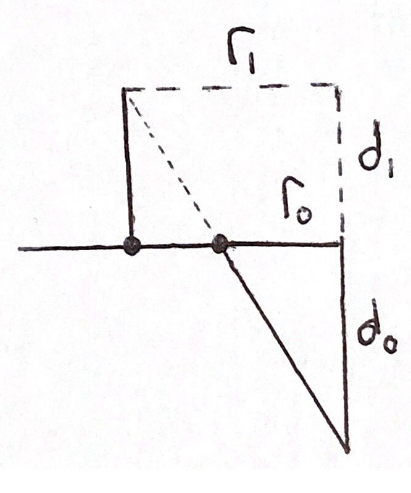
\includegraphics[width=100mm]{dilation_pic.png}
\end{center}

We derive that \(r_{1}\) = \(r_{0}\)\sfrac{\(d_{1}\)}{\(d_{0}\)} because the real and virtual distances form similar triangles. Note that \(d_{0}\) is not very important because it is constant. We first produce the following pattern as a matrix representing all the \(r_{0}\) values:

\begin{center}

\includegraphics[width=100mm]{eye_distances.png}
\end{center}

Note that this is just a linear decay away from the eye. We utilize element-wise multiplication by the depth map to get the virtual distances of every pixel in the image. Finally, we create two "larger" matrices of all zeros and loop through the 2D image pixel by pixel. We fill in each pixel value we loop through at the correct position in the "larger" left and right matrices according to the left and right eyed depths.

The only problem is that this mapping is not mathematically surjective (onto). This results in dark line patterns that run down the image; to fix this, we sacrifice some image resolution. For a 2D signal, a 2D Gaussian distribution acts as a low-pass filter under 2D convolution (equation 56). We convolve the noisy image with a Gaussian of \(\sigma\) = 2 to arrive at our final stereoscopic pairs.

The following image and depth map:

\begin{center}
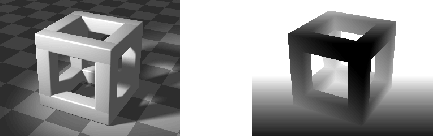
\includegraphics[width=100mm]{image_depth_pair.png}
\end{center}

Turns into:

\begin{center}
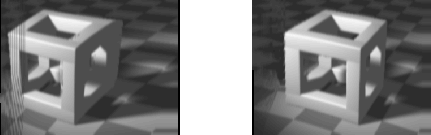
\includegraphics[width=100mm]{stereoscopic_pair.png}
\end{center}

If one zooms into the above image, and follows the instructions detailed on this page: https://www.kula3d.com/how-to-use-the-cross-eyed-method, one should be able to view a 3D cube. (Note the link does not use a finger to focus on, but I recommend using a finger to adjust the focal-depth).

Finally, we captured image and depth information from goggles on the Kinect:

\begin{center}
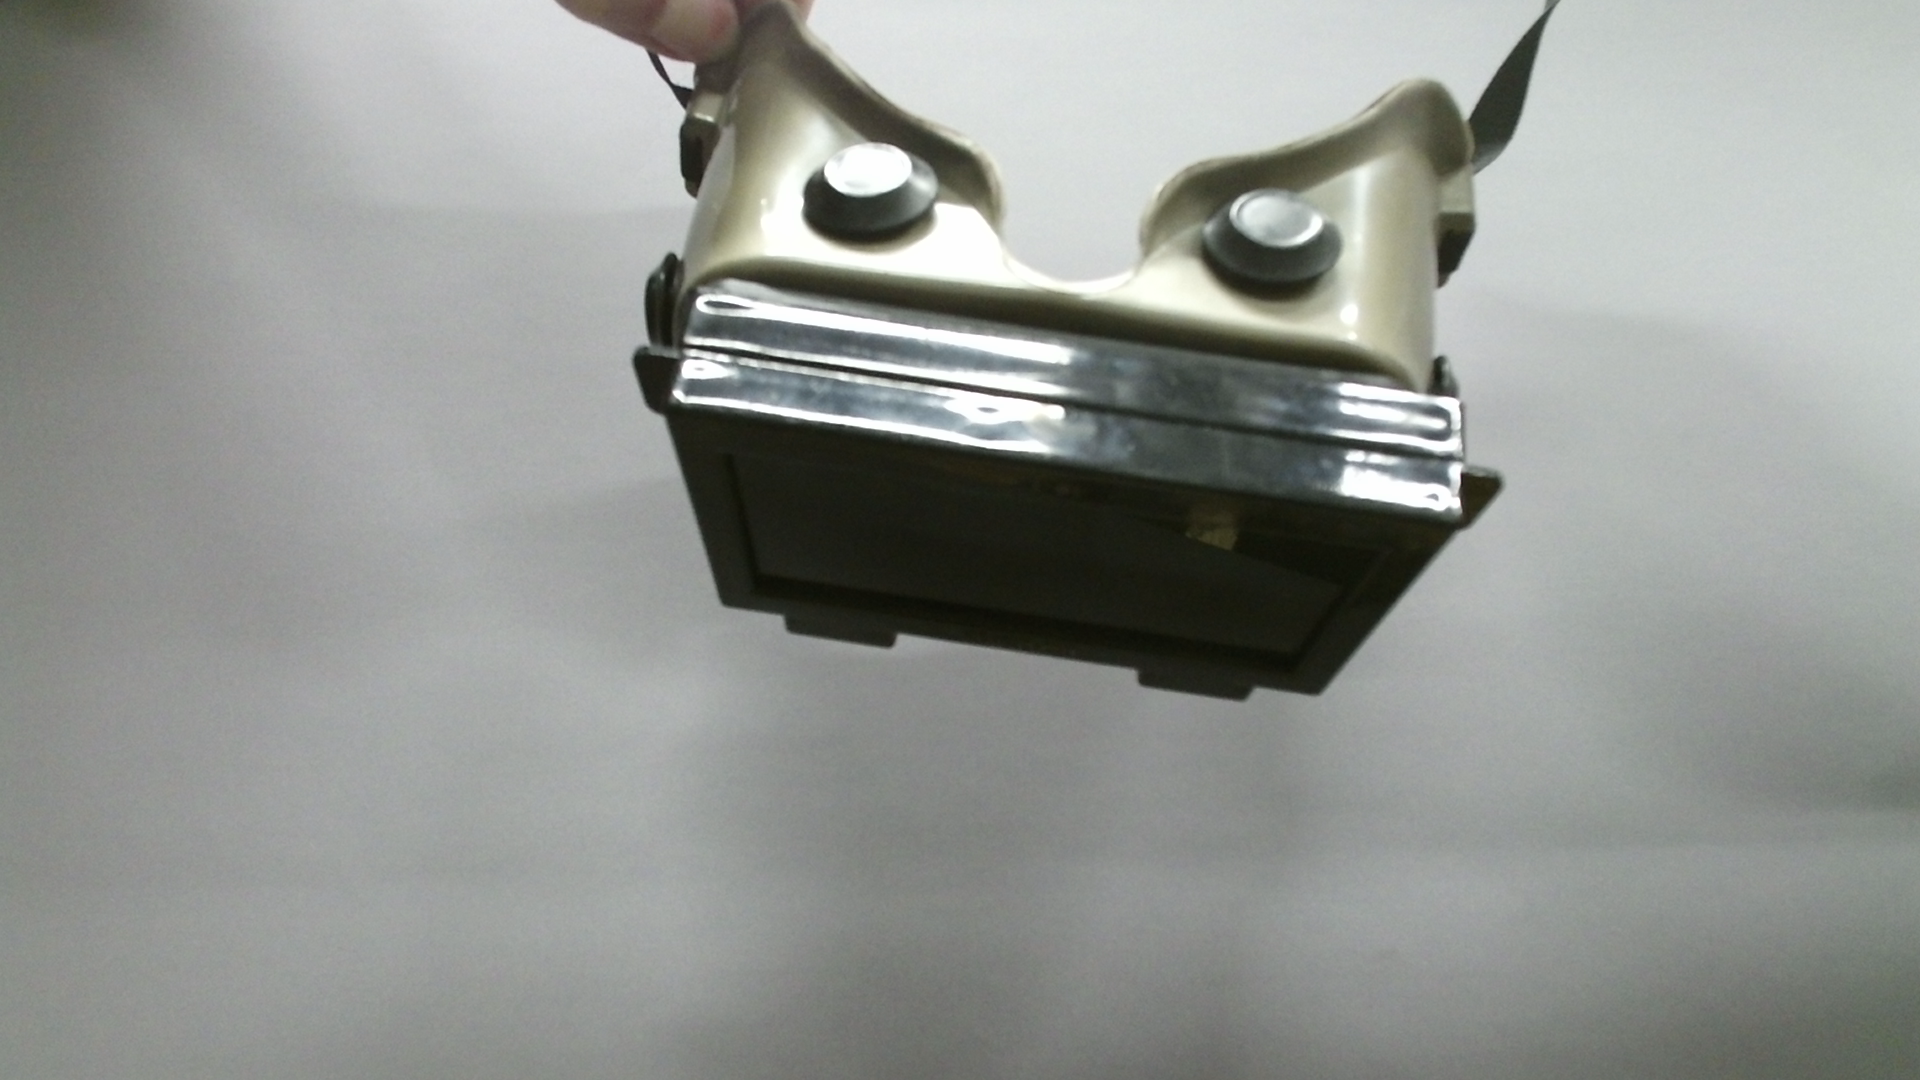
\includegraphics[width=100mm]{goggles.png}
\end{center}

Generated the stereoscopic pairs:

\begin{center}
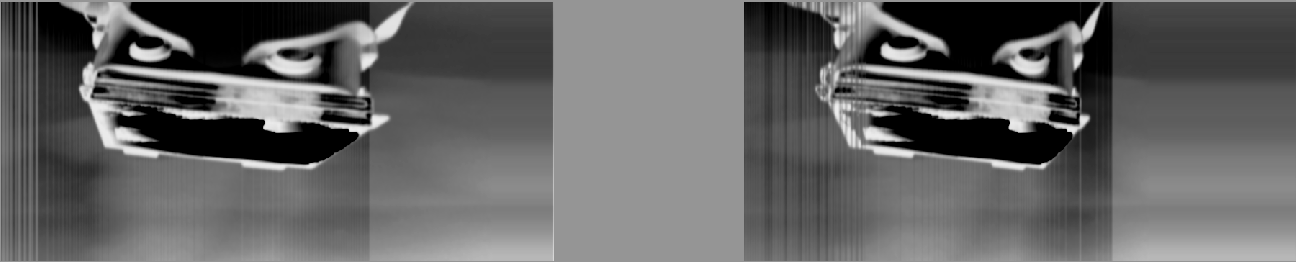
\includegraphics[width=100mm]{goggle_stereoscopic.png}
\end{center}

and turned it into the following output from the SLM:

\begin{center}
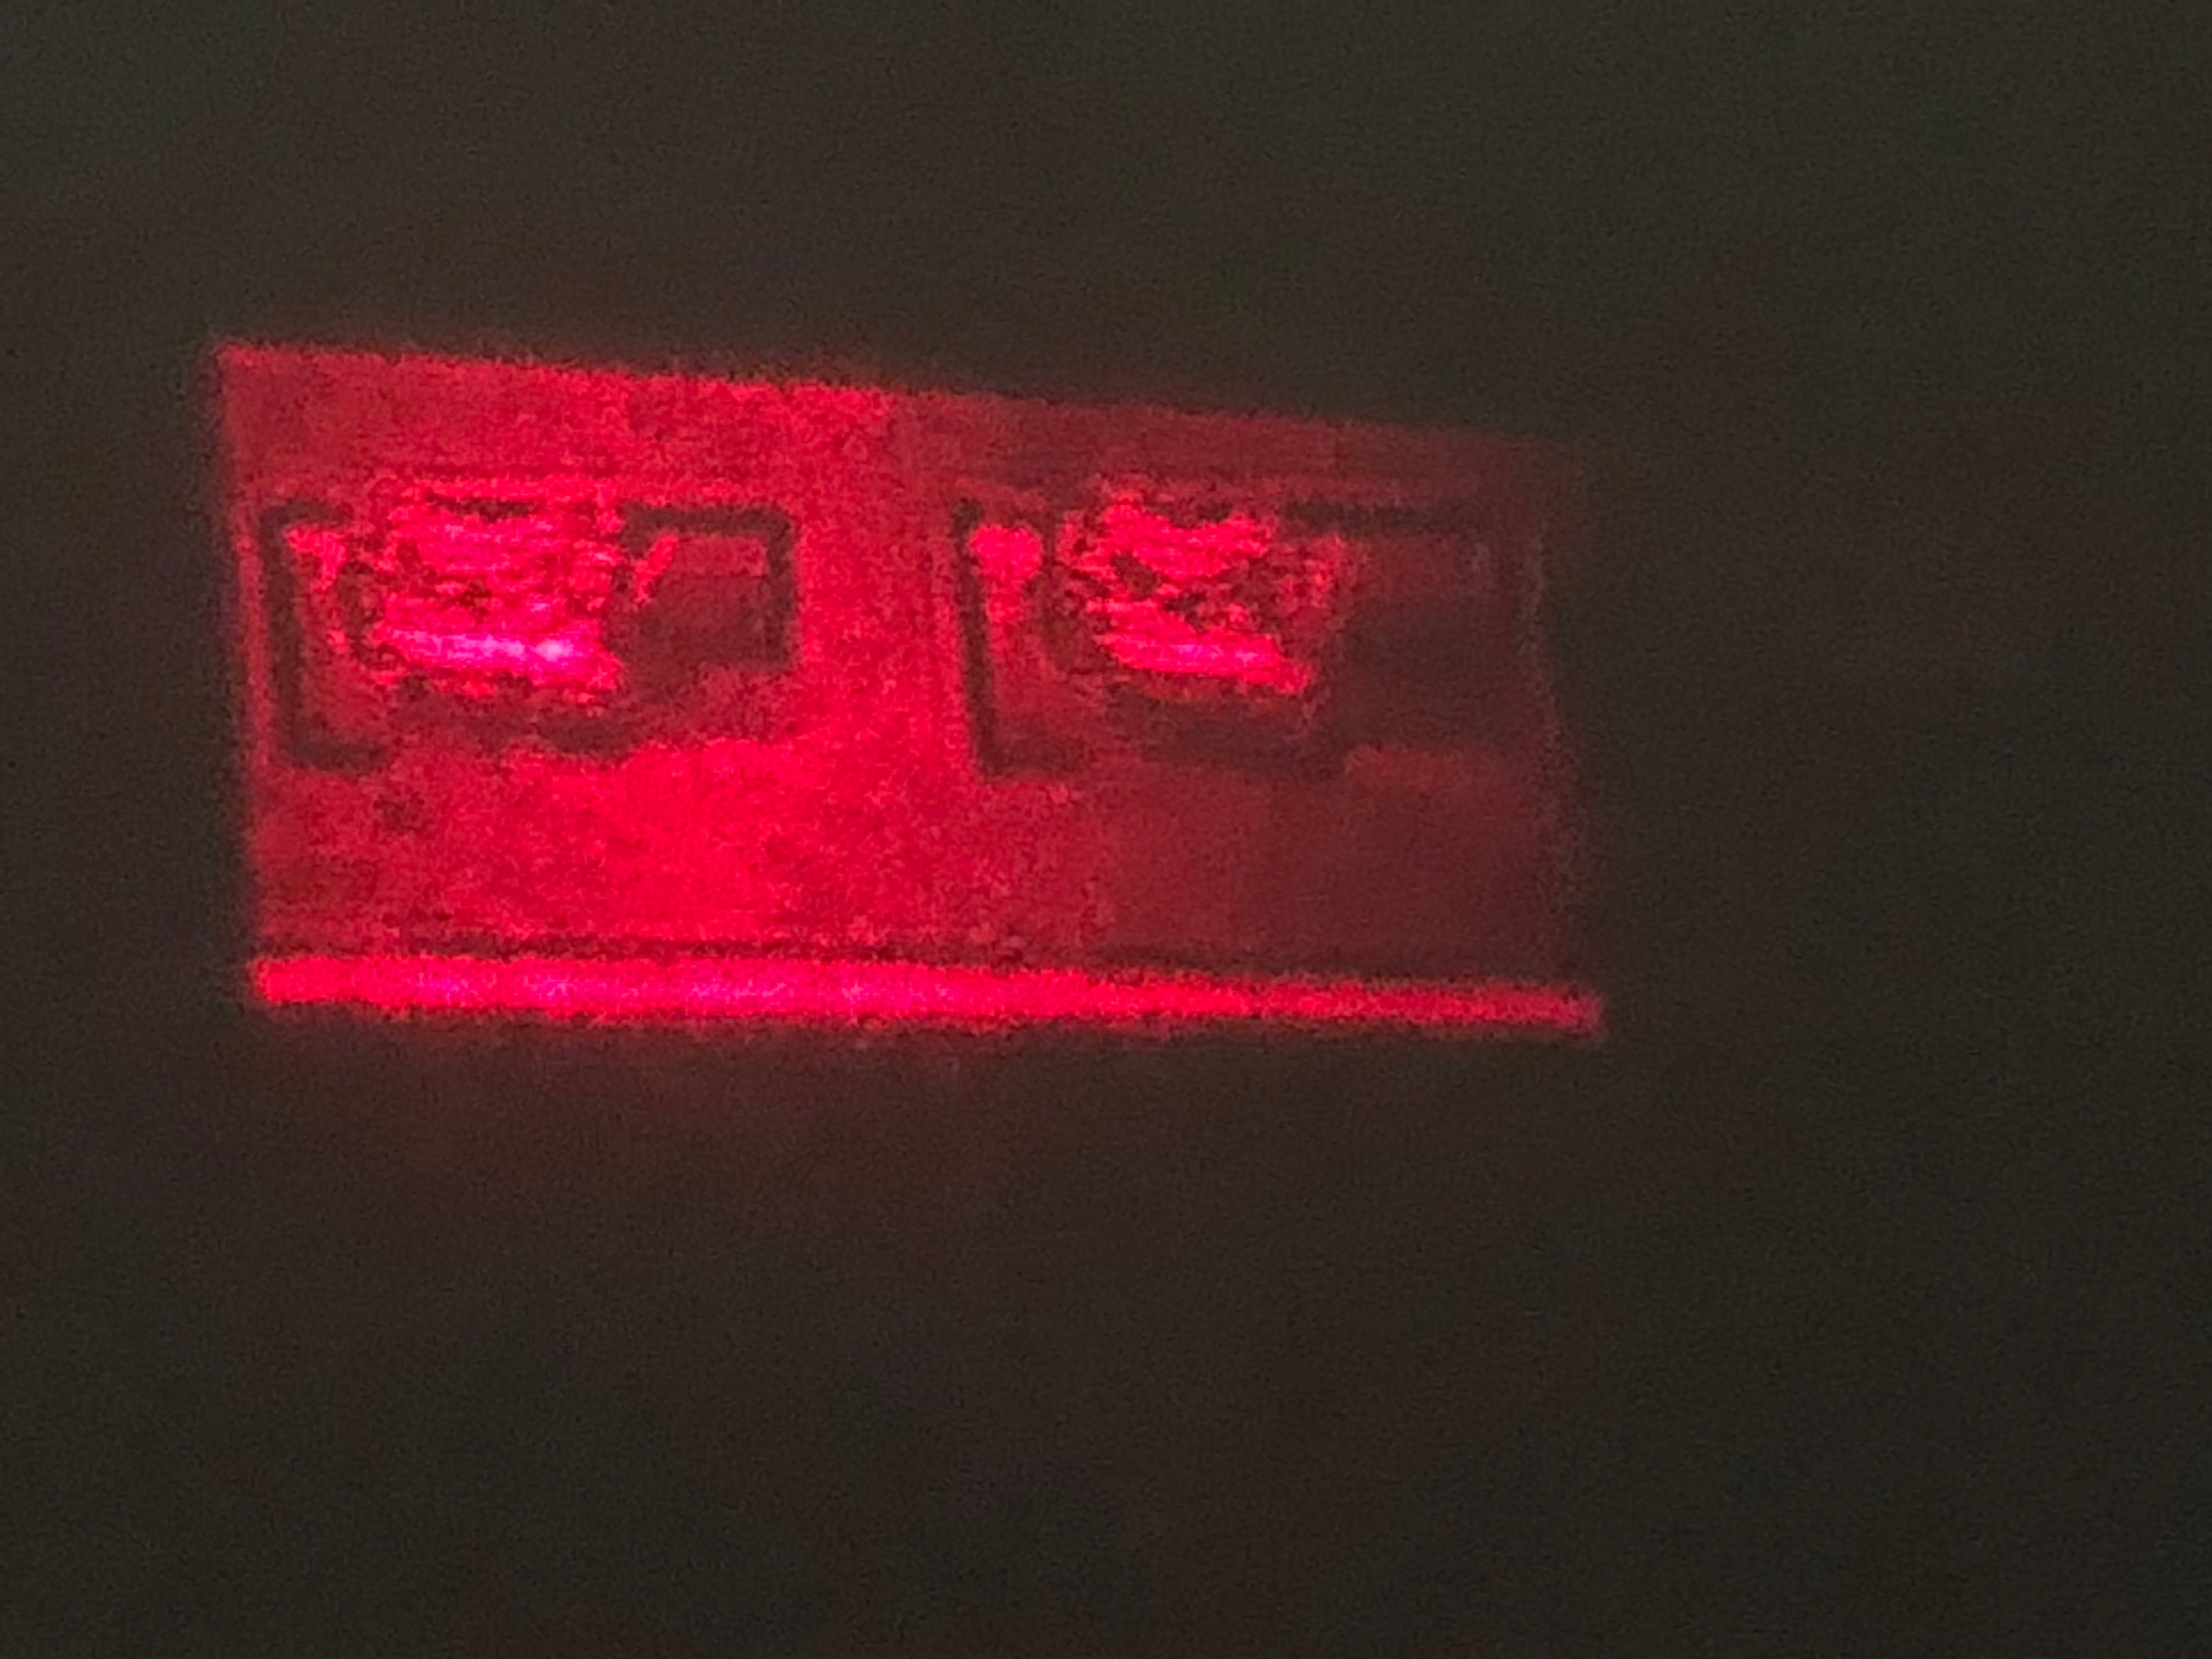
\includegraphics[width=100mm]{final_hologram.jpg}
\end{center}

Once again, the focusing technique can be used to visualize a 3D pair of the goggles. Ben and Ostap in particular noticed that the mind naturally cleans up some of the noise artifacts when viewed in 3D (information loss in one image is alleviated by the other image possessing it).

\section{Status}
Our progress of the project so far was greatly hindered by materials that we need not arriving due to the Canada Post strike. However, we have started setting up the system at the lab, and we feel confident that the hologram system would work with our knowledge. On the software side of the project, the program that converts images into inputs appropriate for the spatial light modulator (SLM) is implemented in two different algorithms. In addition, the Windows Presentation Foundation application that guides the transportation of the Microsoft Kinect images or videos into the SLM is implemented and waiting for testing.

It has been tested that the digital projection stage of the SLM assisted by slmPy module works flawlessly on a computer monitor. The desired image in the form of numpy array is automatically resized to fit the entire screen, and both still image and animation are displayed without any issue. However, additional testing on the SLM is yet to be done as the setup was not completed for projection.

\section{Future goals}
For the upcoming semester, as all the materials have finally arrived, we will be building the holography system, and starting the necessary tests to pick the optimal algorithms for image conversion, resolutions, and sample methods. We hope to be done with the building of the system and getting a complete hologram image by late February so that we can concentrate on making the holography to look more 3D like, and presented in real-time. Currently, another missing piece of the system is the program that encodes the depth information appropriately into the 2D images. Our system inherently deals with 2D images, and the only way to encode the depth information to imbue 3D-like characteristics is through simultaneous projection of phase mask and the depth information to the SLM. It is currently unknown if naively projecting them at the same time will work or additional measures need to be taken. Moreover, it is also important to figure out if we have successfully encoded the depth information without seeing the desired holography, because encoding the depth information is necessary but may not be sufficient for our final goal. These will be the top priorities to be addressed in the upcoming semester.

While we are currently utilizing the IFTA algorithm, it is more computationally intensive than the other algorithm Poon proposes in his book. The other algorithm accounts for the Spatial Distortion that occurs from Fresnel Diffraction and thus premultiplies by the transfer function's inverse to cancel the aperture effects. We will try and get a working prototype with the IFTA algorithm first, but we can speed up computations with this other algorithm if it needed.

For the projection stage, as there is an apparent difference between the SLM reflective surface and a computer monitor, we hope to thoroughly test it the upcoming semester. While the automatically scaled image to fit the computer screen showed no issue, it should also be tested whether such adjustments potentially disturb the quality of holography. After confirmation of reliable projection, we hope to figure out how manipulating certain settings, e.g. the frequency and intensity of the laser beam, refresh rate of the screen, would incur qualitative changes to the projection.

\bibliographystyle{unsrt}
\bibliography{ref}

\end{document}
